\documentclass{article}

% Language setting
% Replace `english' with e.g. `spanish' to change the document language
\usepackage[english,russian]{babel}
\usepackage{amsmath}

%графика
\usepackage{wrapfig}
\usepackage{graphicx}
\usepackage{pgfplots}
\usepackage{tikz}


\usepackage{tcolorbox}

% Set page size and margins
% Replace `letterpaper' with `a4paper' for UK/EU standard size
\usepackage[letterpaper,top=2cm,bottom=2cm,left=3cm,right=3cm,marginparwidth=1.75cm]{geometry}

% Useful packages
\usepackage{amsmath}
\usepackage{amssymb}
\usepackage{graphicx}
\usepackage{fixltx2e}
\usepackage[colorlinks=true, allcolors=blue]{hyperref}

\usepackage{geometry}
\geometry{left=25mm,right=25mm,
 top=25mm,bottom=25mm}

\title{Web3.\\
Lectures. Week 3. \\
Fixed income securities defining elements.\\
Базовые инструменты с фиксированной доходностью.}
\author{Balgabaev Dmitry}

% Колонтитулы
\usepackage{fancyhdr}
\pagestyle{fancy}
\renewcommand{\headrulewidth}{0.1mm}  
\renewcommand{\footrulewidth}{0.1mm}
\lfoot{}
\rfoot{\thepage}
\cfoot{}
\rhead{CMF-2022}
\chead{}

\begin{document}
\maketitle

% Оглавление
\setcounter{tocdepth}{1} % {2} - в оглавлении участвуют chapter, section и subsection. {1} - только chapter и section
\renewcommand\contentsname{Contents}
\tableofcontents
\newpage

\renewcommand{\labelitemi}{\tiny$\bullet$}
\renewcommand{\figurename}{Fig.}
\begin{itemize}
    \item Fixed-income security - финансовые инструменты с фиксированной доходностью, в случае данной лекции - облигации
     \item Bond - Облигация - долговая, эмиссионная ценная бумага
     \item Issuer - Эмитент - организация, которая выпускает свои собственные ценные бумаги
     \item Tenor - время до истечения срока облигации
     \item Principal - конечный платеж облигации
\end{itemize}
 \section{Схема размещения облигаций}
 \begin{figure}[h]
    \centering    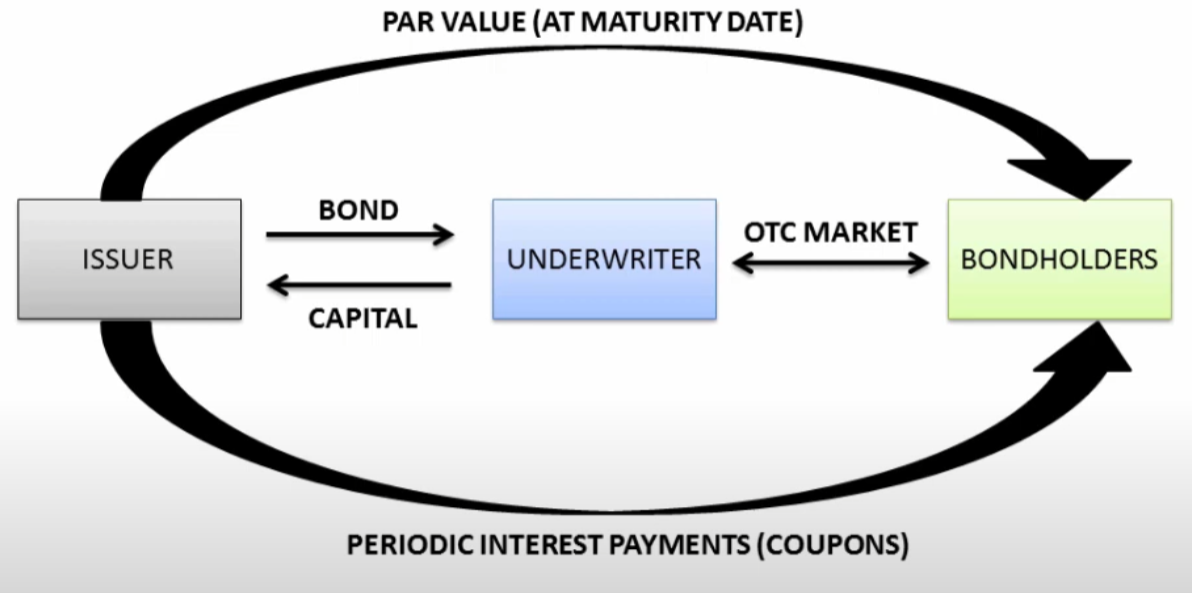
\includegraphics[width=1\textwidth]{scheme1.png}
\end{figure}
\begin{itemize}
    \item {}Компания (issuer) обращается к инвестиционному банку (underwriter)
    \item Инвестиционный банк оценивает заинтересованность инвесторов по доходности с учетом тех рисков, которые представляет заёмщик
    \item Оценивается процентный доход, который нужно будет платить по этому долгу
    \item Выпускается облигация
    \item Инвестиционный банк выкупает все эти облигации и размещает их среди инвесторов
    \item Платежи по этой ценной бумаге прихоядт инвесторам
\end{itemize}

\newpage
\section{Характеристики инструментов с фиксированной доходностью}
Облигации могут быть классифицированны по следующим характеристикам:
\begin{itemize}
    \item Issuer - Эмитент
    \item Maturity date - Дата погашения
    \item Par value - Размер основной суммы долга
    \item Coupon rate - Купонная ставка - какой процент от номинала будет выплачиваться на протяжении долга
    \item Payment frequency - с какой частотой будет выплачиваться купонный доход
    \item Currency denomination - валюта, в которой ценная бумага будет номинирована
\end{itemize}
\begin{flushleft}
\subsection{Виды  \textbf{эмитентов}:}
\end{flushleft}
\begin{itemize}
    \item Наднациональные организации
    \item Государства, муниципальные государства
    \item Квазигосударственные организации
    \item Корпорации:
    \begin{itemize}
        \item Финансовые 
        \item Не финансовые
    \end{itemize}
\end{itemize}
\subsection{Виды облигаций по \textbg{дате погашения}:}
\begin{itemize}
    \item Money market bonds - облигации рынка денег - срок <= 1 год
    \item Capital market bonds - облигации рынка капитала - срок > 1 год
    \item Perpetual bonds - бесконечные облигации
\end{itemize}
\subsection{Виды \textbf{купонных ставок}:}
\begin{itemize}
    \item Fixed - Фиксированный
    \item Floating - Плавающий - может быть привязан к какому-то индксу (LIBOR) и т.д.
    \item Zero - Нулевая купонная ставка - весь процентный доход придет в конце
\end{itemize}
\subsection{Виды облигаций по \textbf{валюте}:}
\begin{itemize}
    \item Single currency - купонный доход и основной платеж будет в единственной валюте
    \item Dual currency - например купонная ставка в USD, а основной платеж в GBP
    \item Currency option bond - инвестору предоставляется выбор в какой валюте будет погашен долг
\end{itemize}
\section{Облигационное соглашение и его содержание}
\textbf{Облигационное соглашение} - контракт между эмитентом и держателем облигации. Он определяет характеристики облигации, права держателя акции и обязанности эмитента.
Облигационное соглашение содержит:
\begin{itemize}
    \item Имя эмитента
    \item Основная сумма долга
    \item Купонная ставка
    \item Даты платежей
    \item Дата выплаты основной суммы долга
    \item Источники средств для погашения облигации
    \item Залоговое обеспечение, если существует
\end{itemize}
\subsection{Ковенанты}
Ковенанты - это ограничения возлагаемые на эмитента, они содержатся в облигационном соглашении и делятся на два типа:
\begin{itemize}
    \item Affirmative - Утвердительные - требуеют определенных действий от эмитента
    \begin{itemize}
        \item Делать все платежи в срок 
        \item Поддерживать залоговое обеспечение на определенном уровне
        \item Поддерживать финансовые показатели на определенном уровне
    \end{itemize}
    \item Negative - Отрицательные - возгалают ограничения на заемщика
    \begin{itemize}
        \item Ограничение на выплату дивидентов
        \item Ограничение на дополнительный долг
        \item Ограничение на залоговое обеспечение
        \item Ограничение на продажу активов
    \end{itemize}
\end{itemize}
\section {Юридические, регуляторные и налоговые положения, которые влияют на процесс эмиссии и торговли облигациями}
Облигации могут быть выпущены на:
\begin{itemize}
    \item Домашнем рынке
    \item Иностранном рынке
    \item Рынке еврооблигаций (менее зарегулирован, не ведется реестр конечных владельцев)
\end{itemize}
Регуляторные положения указаны в облигационном соглашении и содержат в себе информацию о:
\begin{itemize}
    \item Эмитенте
    \item Источниках погашения долга
    \item Залогом обеспечении
    \item Гаранторах
    \item Банковских аккредитивах и т.д
\end{itemize}
\subsection{Налогооблажение}
В различных странах налогообложение отличается, облагается:
\begin{itemize}
    \item Стоимость облигации
    \item Периодические платежи 
\end{itemize}
\begin{itemize}
    \item [--]Эти ставки в различных странах могут как совпадать, так и отличаться
    \item [--]\textbf{Государственные} облигации налогами не облагаются 
    \item [--]Облигации с долгим сроком погашения облагаются меньше, чем облигации с коротким сроком погашения
\end{itemize}
\section{Денежные потоки инструментов с фиксированной доходностью}
Следует помнить, что инструменты с фиксированной доходностью - это только название, которое определяет целый класс финансовых инструментов, доход по ним не всегда фиксированный.
\subsection{Виды облигаций по \textbf{выплате основной суммы долга}}
\begin{itemize}
    \item Bullet structure - вся сумма придет в конце
    \item Amortized structure - периодические выплаты как купонов, так и основной суммы долга
    \item Sinking fund arrangement - Амортизационный фонд - обязательство эмитента создать фонд, откладывать туда деньги и с помощью этого фонда выкупать часть облигаций с рынка
\end{itemize}
\subsection{Виды \textbf{купонов}}
\begin{itemize}
    \item Floating-rate notes - купоны могут быть привязаны к какой-то ставке 
    \item Index-linked bonds - купоны могут быть привязаны к какому-то индексу (если облигация индкесируется на индекс инфляции, у нее корректируется номинал, но так, как купон - это процент от номинала, купон тоже изменит свою цену)
    \item Step-up notes - купонная ставка первое время постоянна, а затем начинает увеличиваться (например, какая-то организация наращивает производственные мощности)
    \item Payment-in-kind (PIK) bonds - вместо выплаты деньгами, платежи по облигации производятся этими же облигациями (например, компания находится в дефолтном состоянии)
\end{itemize}
\newpage
\section{Условные положения, которые влияют на срок и природу денежных платежей в инструментах с фиксированной доходностью}
В облигацию могут быть встроены:
\begin{itemize}
    \item Put опцион - право инвестора потребовать досрочное погашение долга (зачастую, это условное право, которое включается, если эмитент нарушил какой-то ковенант)
    \item Call опцион - право эмитента досрочно погасить свой долг (компания занимает под какую-то ставку, но считает, что она высокая, когда ставка упадет, компания отзовет свои облигации, и займет новые облигации, под меньший процент)
    \item Опцион на обмен облигации на определенное колличество акций компании (\textbf{convertible bonds}) (после использования опциона облигация исчезает)
    \item Warrant - поверх облигации есть опцион (после использования опциона облигация не исчезает)
\end{itemize}
\end{document}
